\documentclass[aspectratio=169,11pt]{beamer}

\usepackage{graphicx}
\usepackage{booktabs}
\usepackage{amsmath,amssymb}
\usepackage{tikz}
\usetikzlibrary{arrows.meta,positioning}

% reuse the paper's figures and logo, nothing is regenerated.
% first hit wins, so a local figures/ overrides the paper's.
\graphicspath{{figures/}{../paper/figures/}}

\usepackage{loomtheme}

% notebook-generated table bodies from the paper; the primitive input lets \bottomrule follow
\makeatletter\newcommand{\tablebody}[1]{\@@input ../paper/tables/#1.tex }\makeatother

\title{Algorithmic Analysis of Water Distribution Networks}
\subtitle{TC2038 Situation Problem 2: all seven tasks}
\author{Santiago Hernández Senosiain}
\date{November 2, 2026}

\begin{document}

\begin{frame}[plain]
  \centering
  
\includegraphics[height=1.1cm]{tec_logo.png}\\[1.2em]
  {\usebeamerfont{title}\usebeamercolor[fg]{title}\inserttitle\par}
  \vspace{0.3em}{\large\insertsubtitle\par}
  \vspace{1.2em}{\insertauthor\par}
  \vspace{0.3em}{\small\insertdate\par}
\end{frame}

\begin{frame}{Outline}
  \tableofcontents
\end{frame}

\section{Problem}
\begin{frame}{Problem}
  \begin{itemize}
    \item what is broken, in one line
    \item why it matters
  \end{itemize}
  \note{notes: the prose from the paper's introduction goes here}
\end{frame}

\section{Methods}
\begin{frame}{Methods}
  \begin{itemize}
    \item the approach in one line, keep this frame tight
  \end{itemize}
  \note{notes: derivations and detail stay spoken, not on the slide}
\end{frame}

\section{Findings}
\begin{frame}{T1 and T2: representation and lengths}
  \begin{itemize}
    \item Matrix BFS 8 to more than 20 times slower than the list; matrix memory twice the list on PES
    \item Matrix only wins the pipe-existence query: used only for all-pairs tables
    \item Length and capacity are distinct attributes (correlation $-0.65$ to $+0.13$)
    \item Network distance is 19\% (FOS) to 83\% (PES) longer than straight-line on average
    \item PES: nodes 19 and 39 are 147 apart, 4,146 by pipe (two clusters, few links)
  \end{itemize}
  \note{The networks are so sparse that a matrix wastes almost every cell. Circuity explains later results: PES's two clusters are why only two pipes separate its sectors.}
\end{frame}

\begin{frame}{T3 and T4: sectors and the oldest water}
  \begin{columns}[c]
    \begin{column}{0.6\textwidth}
      \centering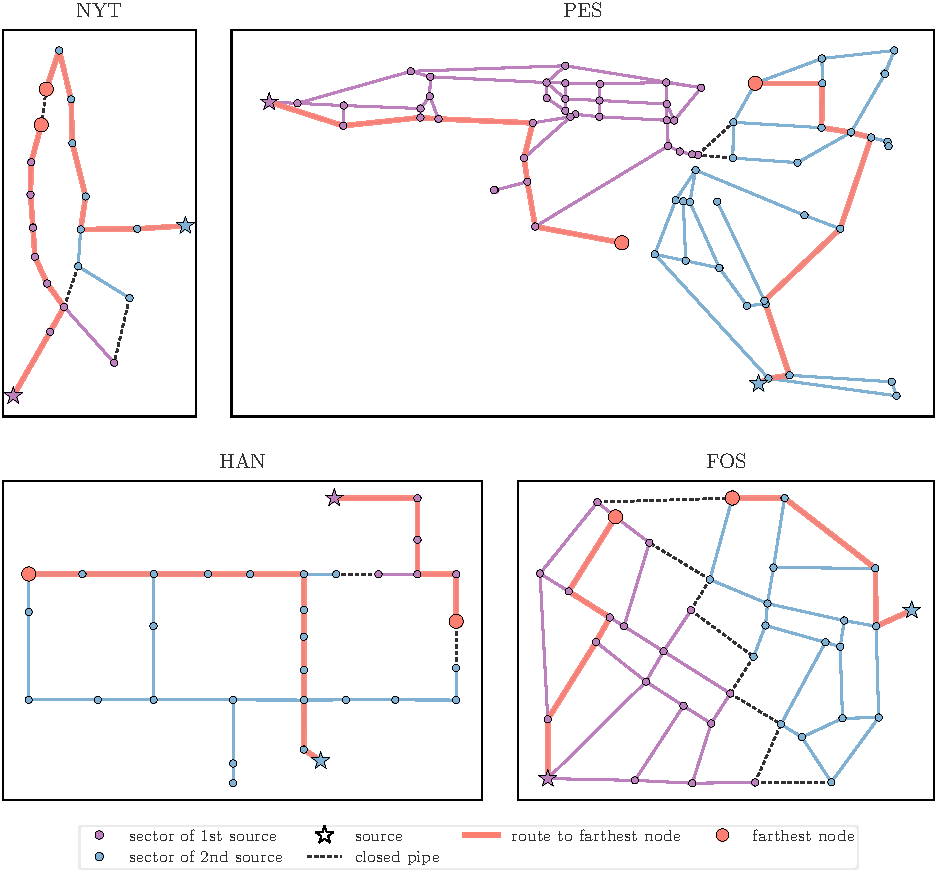
\includegraphics[height=0.76\textheight]{freshness.pdf}
    \end{column}
    \begin{column}{0.38\textwidth}
      \small
      \begin{itemize}
        \item Pipes to close: 3 (NYT), 2 (HAN), 8 (FOS), 2 (PES)
        \item Multi-source: half the relaxations of per-source Dijkstra
        \item 4 of 8 farthest nodes sit at a closed pipe
        \item Sectors cut a source's worst water age by up to 2.75 times (HAN 13)
      \end{itemize}
    \end{column}
  \end{columns}
  \note{The farthest node of each sector is where water is oldest, the natural monitoring point. Closing the boundary pipes never lengthens a node's route to its own source.}
\end{frame}

\begin{frame}{T5: shortest route is not maximum flow}
  \centering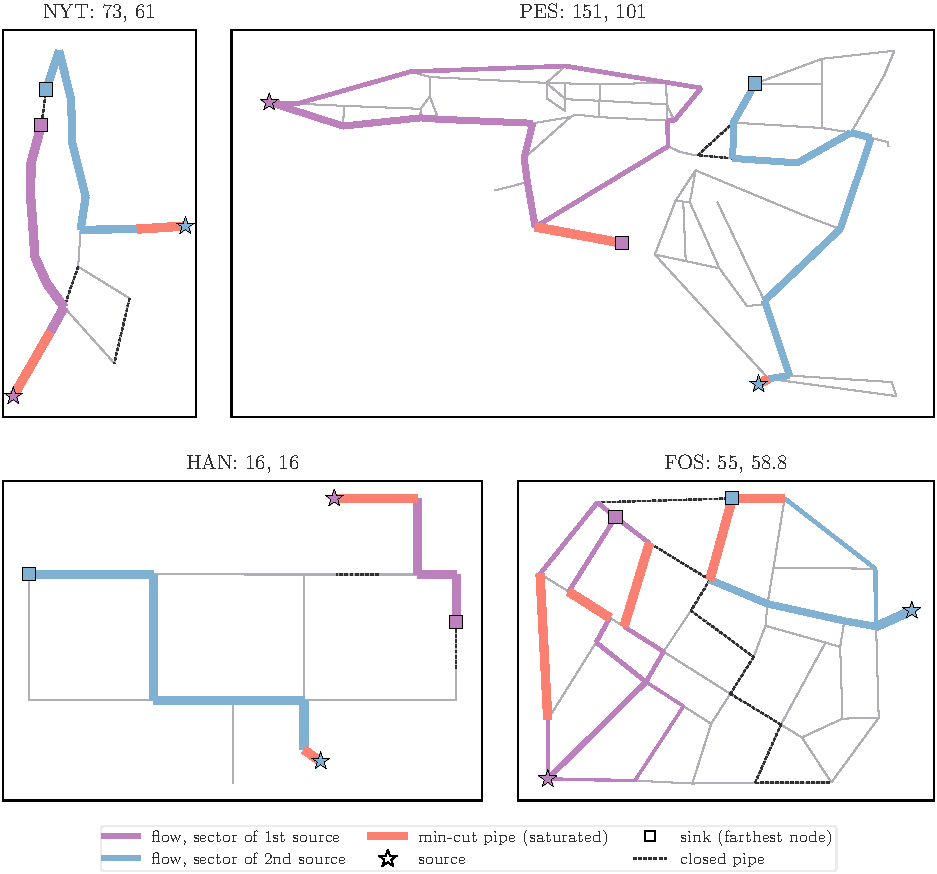
\includegraphics[height=0.5\textheight]{flows.pdf}\par\raggedright
  \small
  \begin{itemize}
    \item 6 of 8 sectors: the min cut is the single pipe at a leaf source or sink
    \item FOS: three bottleneck pipes carry 55, the shortest route alone 19; PES 1: 151 vs 101
    \item Unlimited cut pipes: no gain in HAN (chains of 16), up to 3.6 times in FOS
  \end{itemize}
  \note{Same source-sink pairs as T4. The route minimises length; the flow is set by the narrowest cut across all routes. Edmonds-Karp and Dinic always agree, with at most four augmenting paths.}
\end{frame}

\begin{frame}{T6: sampling routes}
  \centering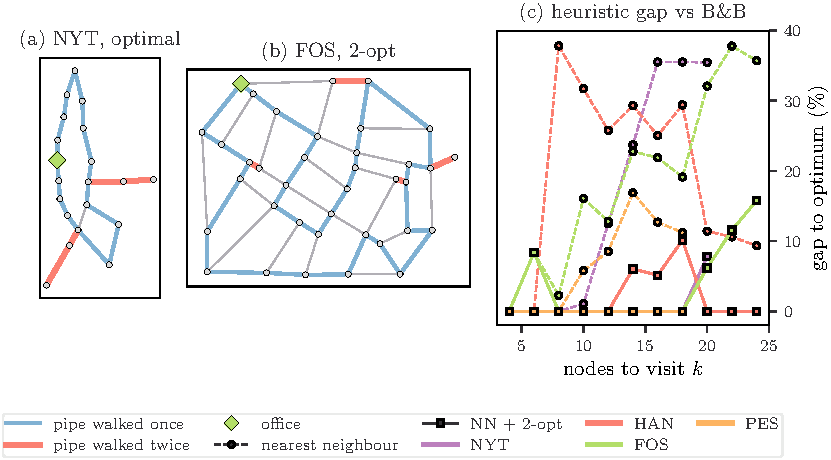
\includegraphics[height=0.56\textheight]{routes.pdf}\par\raggedright
  \small
  \begin{itemize}
    \item NYT optimal (7,072, proven by branch and bound); HAN, FOS, PES approximate
    \item 40 subsets with known optimum: NN 16.0\% above, NN + 2-opt 1.9\%, optimal in 31
  \end{itemize}
  \note{Pipes walked twice are the dead ends. The MST bound is too weak to certify the larger instances, so only NYT and subsets up to 26 nodes are proven.}
\end{frame}

\begin{frame}{T6 extension: a selection hyper-heuristic}
  \centering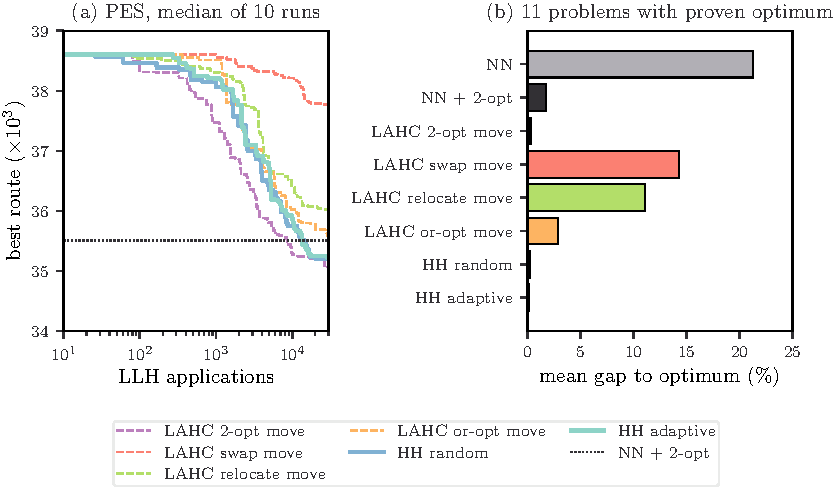
\includegraphics[height=0.52\textheight]{hyperheuristic.pdf}\par\raggedright
  \small
  \begin{itemize}
    \item Each step picks one random move (2-opt, swap, relocate, or-opt); late acceptance (LAHC); 30,000 steps, 10 seeds
    \item 0.2\% mean gap on 11 solved problems vs 0.29\% for the best single move (LAHC 2-opt move); best HAN and FOS route in 9 and 6 of 10 runs (vs 3 and 2)
    \item Best PES route of the study: 34,700, 2.3\% below the T6 route
  \end{itemize}
  \note{A hyper-heuristic searches over heuristics instead of solutions. Its gain here is consistency. The adaptive rule ended up nearly uniform: near a local optimum all moves rarely improve, so their credit decays to the same floor.}
\end{frame}

\begin{frame}{T7: expansion}
  \begin{columns}[c]
    \begin{column}{0.58\textwidth}
      \centering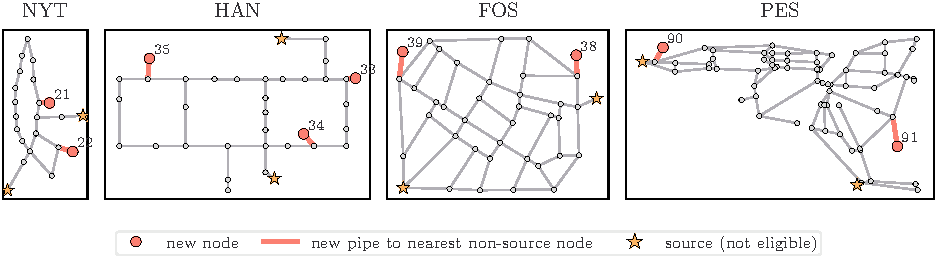
\includegraphics[height=0.8\textheight]{expansion.pdf}
    \end{column}
    \begin{column}{0.4\textwidth}
      \small
      \begin{itemize}
        \item Each new node links to its nearest non-source node
        \item FOS point $(7071, 9055)$ becomes node 38 linked to node 17, as in the challenge slides
        \item 2-d tree checks 6.7 of 18 candidates (NYT) and 11 of 69 (PES) per query
        \item List update writes 3 entries; matrix copies the whole table
      \end{itemize}
    \end{column}
  \end{columns}
  \note{Every connection matches brute force and SciPy. With two or three insertions per instance brute force is enough; the tree pays for its build only after a few tens of queries.}
\end{frame}

\begin{frame}{Performance against theory}
  \begin{columns}[c]
    \begin{column}{0.6\textwidth}
      \centering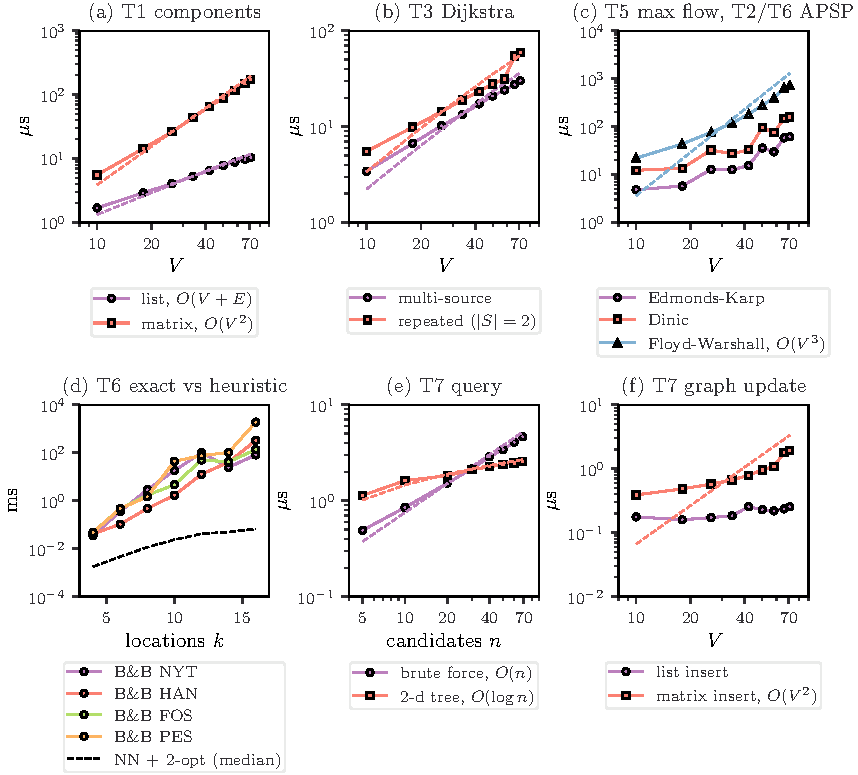
\includegraphics[height=0.8\textheight]{performance.pdf}
    \end{column}
    \begin{column}{0.38\textwidth}
      \small
      \begin{itemize}
        \item List $\sim V+E$, matrix $\sim V^2$, Dijkstra $\sim (V+E)\log V$
        \item Floyd-Warshall below $V^3$: NumPy overhead at $V\le 71$
        \item Flows far below worst case: at most 4 augmentations
        \item Branch and bound: about 1.4 to 2.2 times per added location
      \end{itemize}
    \end{column}
  \end{columns}
  \note{Growth was measured on subsets because four instances are too few. Branch and bound is the only cost that explodes.}
\end{frame}

\section{Connections}
\begin{frame}{How the tasks inform each other}
  \centering
  \begin{tikzpicture}[node distance=0.5cm and 0.6cm, every node/.style={font=\small},
      box/.style={draw=loomaccent, fill=loomaccent!12, rounded corners=2pt, minimum width=1.9cm, minimum height=0.7cm, align=center},
      arr/.style={-{Stealth[length=2mm]}, loomink, thick}]
    \node[box] (t1) {T1\\representation};
    \node[box, right=of t1] (t2) {T2\\lengths};
    \node[box, right=of t2] (t3) {T3\\sectors};
    \node[box, right=of t3] (t4) {T4\\farthest node};
    \node[box, right=of t4] (t5) {T5\\max flow};
    \node[box, below=of t3] (t6) {T6\\sampling route};
    \node[box, below=of t6] (t7) {T7\\expansion};
    \draw[arr] (t1) -- (t2);
    \draw[arr] (t2) -- node[above, font=\scriptsize] {$\ell$} (t3);
    \draw[arr] (t3) -- node[above, font=\scriptsize] {$V_s$} (t4);
    \draw[arr] (t4) -- node[above, font=\scriptsize] {$t_s$} (t5);
    \draw[arr] (t2) |- node[pos=0.25, left, font=\scriptsize] {metric closure} (t6);
    \draw[arr] (t7) -| node[pos=0.25, below, font=\scriptsize] {changes the network} (t1);
  \end{tikzpicture}
  \vspace{0.5em}
  \begin{itemize}\small
    \item Leaf sources explain the there-and-back legs (T6) and five of the six single-pipe bottlenecks (T5)
    \item PES's two clusters (T2) explain why two closures separate its sectors (T3)
    \item Same source-sink pairs: shortest route (T4) vs narrowest cut (T5)
  \end{itemize}
  \note{One package function chain feeds every notebook, so the sectors, farthest nodes and sinks are identical everywhere.}
\end{frame}

\section{Conclusions}
\begin{frame}{Conclusions and limitations}
  \begin{itemize}
    \item T6 is the only hard problem: exponential exact search, optimum proven only for NYT and subsets up to 26 nodes
    \item Cheap heuristics carry most of the value: NN + 2-opt 1.9\% above the optimum on average; the hyper-heuristic adds consistency
    \item Most expensive polynomial step: Floyd-Warshall, $O(V^3)$; everything else is near linear here
  \end{itemize}
  \vspace{0.4em}
  \textbf{Limitations}
  \begin{itemize}\small
    \item No hydraulics: no pressure, head loss or demand; capacities without units; age $\propto$ distance
    \item One source-sink pair per sector; stated conventions for duplicates, outliers and insertion order
    \item Weak bound on near-trees; small instances, so growth measured on subsets
  \end{itemize}
  \note{The study shows how different techniques answer different questions on the same network, and how the answers explain one another.}
\end{frame}


\begin{frame}[plain]
  \centering
  {\usebeamerfont{title}\usebeamercolor[fg]{title}Thanks\par}
  \vspace{0.5em}{\large Questions?\par}
\end{frame}

\end{document}
